\documentclass[reqno,a4paper,12pt]{amsart}

\usepackage{amsmath,amssymb,amsthm,geometry,xcolor,soul,graphicx}
\usepackage{titlesec}
\usepackage{xeCJK}
\setCJKmainfont{Kai}

\geometry{left=0.7in, right=0.7in, top=1in, bottom=1in}



\renewcommand{\baselinestretch}{1.3}

\title{高等热力学与统计物理第二次作业}
\author{董建宇}


\begin{document}
\maketitle

\titleformat{\section}[hang]{\small}{\thesection}{0.8em}{}{}
\titleformat{\subsection}[hang]{\small}{\thesubsection}{0.8em}{}{}

\section{}
	假设热容量$C_V$为常数,求体积为$V$,温度为$T$的理想气体的熵(确定到一个任意常数),用所得结果和Joule自由膨胀实验论证熵增加原理。 
	\begin{enumerate}
	\item 
	\begin{proof}
	由熵的定义可知:
	\[
		dS = \frac{\delta Q}{T}
	\]
	则理想气体的熵为:
	\[
		S(T, V) = \int \frac{\delta Q}{T} = \int \frac{C_V\,dT}{T} + \int \frac{p}{T}\,dV = C_V\ln T + nR \ln V + S_0.
	\]
	自由膨胀前气体的熵为:
	\[
		S_0(T_0, V_0) = C_V\ln T_0 + nR\ln V_0 + S_0.
	\]
	自由膨胀之后,由热力学第一定律可知,气体温度不变,仍为$T_0$,体积变为$V$$(V>V_0)$,则膨胀后气体的熵为:
	\[
		S(T_0, V) = C_V\ln T_0 + nR\ln V + S_0
	\]
	熵增为:
	\[
		\Delta S = S(T_0, V) - S_0(T_0, V_0) = nR\ln\frac{V}{V_0} > 0.
	\]
	即在孤立系统中,气体绝热自由膨胀这一不可逆过程导致系统的熵增加。
	\end{proof}
\end{enumerate}

\section{}
	某一物质具有下列性质: \\
	在恒定温度$T_0$下从体积$V_0$膨胀到$V$所做的功为:
	\begin{equation*}
		W = RT_0\ln\frac{V}{V_0}.
	\end{equation*}
	该物质的熵由下式给出:
	\begin{equation*}
		S = R\frac{V}{V_0}\left( \frac{T}{T_0} \right)^\alpha.
	\end{equation*}
	其中$T_0$,$V_0$和$\alpha$为固定常数。
\begin{enumerate}
	\item 计算该物质的Helmholtz自由能
	\begin{proof}
%		对熵进行全微分可得:
%		\[
%			dS = \frac{R}{V_0}\left( \frac{T}{T_0} \right)^\alpha\,dV + \frac{RV}{V_0}\frac{\alpha T^{\alpha-1}}{T_0^{\alpha}}\,dT.
%		\]
%		对做功全微分可得:
%		\[
%			dW = \frac{RT_0}{V}\,dV.
%		\]
		由热力学微分关系有:
		\[
			\,dF = -S\,dT - p\,dV.
		\]
		即有:
		\[
			\left( \frac{\partial F}{\partial T} \right)_V = -S = -R\frac{V}{V_0}\left( \frac{T}{T_0} \right)^\alpha.
		\]
		两侧积分可得:
		\[
			F(T, V) = -\frac{RVT^{\alpha+1}}{(\alpha+1)V_0T_0^{\alpha}} + g(V).
		\]
		其中$g(V)$是只与体积$V$有关的函数。满足:
		\[
			\left( \frac{\partial F}{\partial V} \right)_T = -\frac{dW}{dV} = -\frac{RT_0}{V} = \frac{d g(V)}{dV} - \frac{RT_0}{(\alpha+1)V_0}.
		\]
		可以解得:
		\[
			g(V) = -RT_0\ln V + \frac{RT_0V}{(\alpha+1)V_0} + C
		\]
		其中$C$是一个与$T,V$无关的常数。则自由能为:
		\[
			F(T, V) = -RT_0\ln V + \frac{RT_0V}{(\alpha+1)V_0}\left( 1 - \left( \frac{T}{T_0} \right)^{\alpha+1} \right) + C.
		\]
		利用初始条件$F(T_0, V_0)$可计算得$C$,代入上式知:
		\[
			F(T, V) = F(T_0, V_0) - RT_0\ln\frac{V}{V_0} + \frac{RT_0V}{(\alpha+1)V_0}\left( 1 - \left( \frac{T}{T_0} \right)^{\alpha+1} \right).
		\]
	\end{proof}
	
	\item 求该物质的状态方程
	\begin{proof}
		由热力学量微分关系可知状态方程为:
		\[
			p = -\left( \frac{\partial F}{\partial V} \right)T = \frac{RT_0}{V} - \frac{RT_0}{(\alpha+1)V_0} \left( 1 - \left( \frac{T}{T_0} \right)^{\alpha+1} \right)
		\]
	\end{proof}
	
	\item 求在任意恒定温度$T$下体积从$V_0$膨胀到$V$所做的功
	\begin{proof}
		\[
			W = \int_{V_0}^V p\,dV = RT_0\ln\frac{V}{V_0} - \frac{T_0R}{\alpha+1}\left( \frac{V}{V_0}-1 \right)\left( 1 - \left( \frac{T}{T_0} \right)^{\alpha+1} \right).
		\]
	\end{proof}
\end{enumerate}

\section{}
	一热机循环如下边的T-S图所示。其中A代表灰色区域的面积,B代表灰色区域以下至坐标轴的面积。
	\begin{center}
		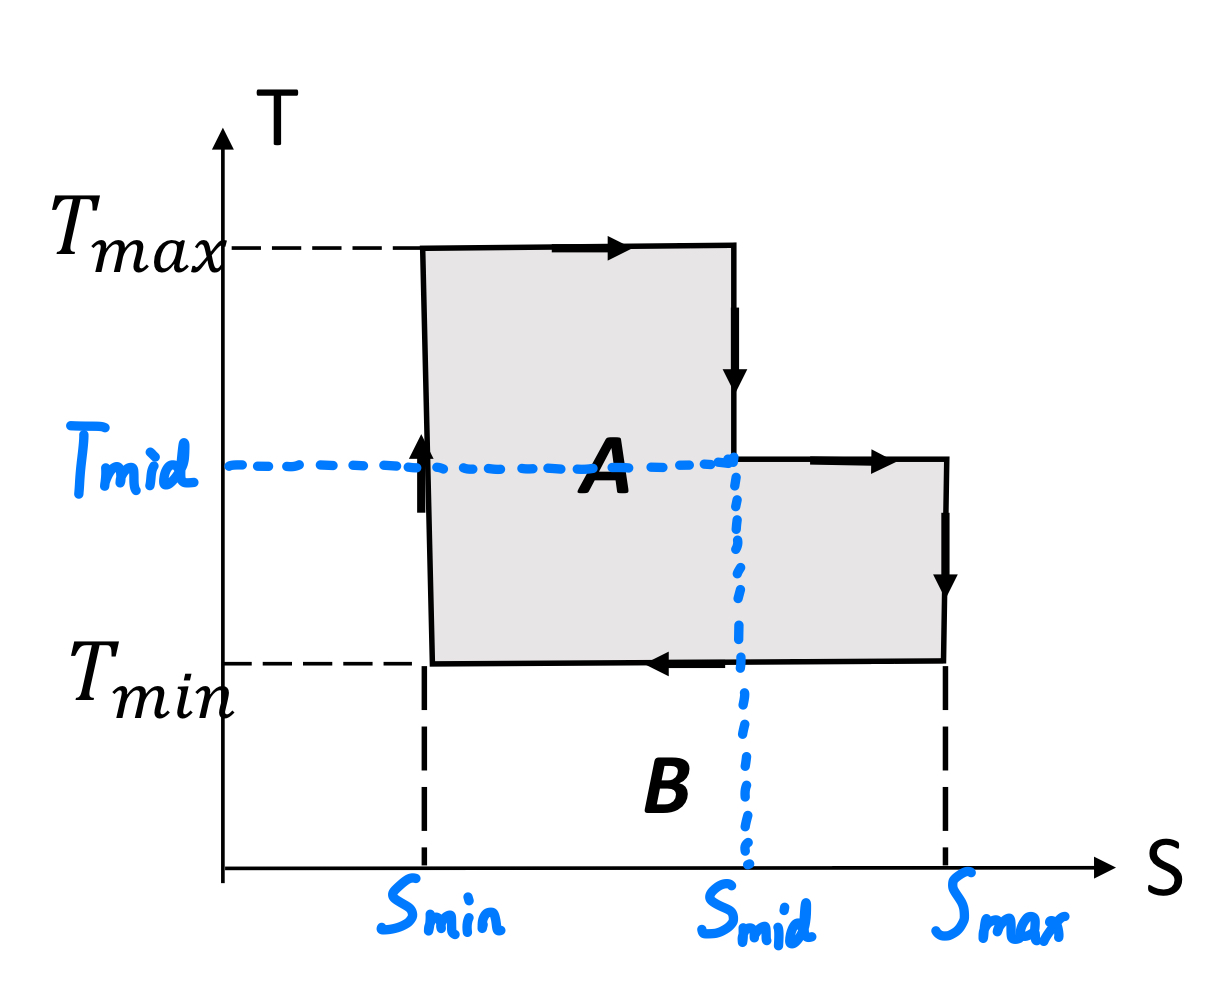
\includegraphics[scale = 0.3]{hw2problem3.jpeg}
	\end{center}
	\begin{enumerate}
		\item 证明此热机循环的效率不可能超过可逆循环的效率.
		\begin{proof}
			对于任意一个热力学过程有:
			\[
				\delta Q \leq T\,dS.
			\]
			当且仅当热机循环可逆式等号成立。对于上图热力学循环吸热过程,积分得:
			\[
				\int \delta Q = Q_1 \leq \oint T\,dS = S_A + S_B
			\]
			其中$Q_1$和$Q_2$表示该热力学循环一次的吸热与放热;$Q_A$与$Q_B$表示可逆循环的吸热与放热。即此热机循环的净吸热小于或等于可逆循环的净吸热。同时,在温度为$T_{min}$熵从$S_{max}$降低到$S_{min}$热力学过程,有:
			\[
				-Q_2 \leq T_{min}(S_{min}-S_{max}) = -S_B.
			\]
%			即有:
%			\[
%				Q_1 \geq Q_A.
%			\]
			则此热机循环的效率$\eta_1 = 1-\frac{Q_2}{Q_1}$与可逆循环的效率$\eta_2 = 1-\frac{S_B}{S_A+S_B}$的关系为:
			\[
				\eta_1 = 1-\frac{Q_2}{Q_1} \leq \eta_2 = 1-\frac{S_B}{S_A+S_B}.
			\]
			当且仅当此热机循环为可逆循环时等号成立。
		\end{proof}

		\item 证明可逆热机的效率不可能超过工作于最高和最低温度,$T_{max}$和$T_{min}$,之间的Carnot热机效率。
		\begin{proof}
			对于可逆热机,有:
			\begin{align*}
				Q_A &= \int T\,dS = \int_{S_{min}}^{S_{mid}} T_{max}\,dS + \int_{S_{mid}}^{S_{max}} T_{mid}\,dS \\ 
				&= T_{max}(S_{mid}-S_{min}) + T_{mid}(S_{max}-S_{mid}), \\
				Q_B &= \int T\,dS = \int_{S_{min}}^{S_{max}} T_{min}\,dS \\
				&= T_{min}(S_{max}-S_{min}).
			\end{align*}
			则可逆热机循环的效率为:
			\[
				\eta_2 = \frac{Q_A-Q_B}{Q_A} = \frac{T_{max}(S_{mid}-S_{min}) + T_{mid}(S_{max}-S_{mid}) - T_{min}(S_{max}-S_{min})}{T_{max}(S_{mid}-S_{min}) + T_{mid}(S_{max}-S_{mid})} < 1.
			\]
			由于$\eta_2<1$,分子分母同时加$(T_{max}(S_{max}-S_{mid}) - T_{mid}(S_{max}-S_{mid}) = (T_{max}-T_{mid})(S_{max}-S_{mid})) > 0$,分数变大即:
			\[
				\eta_2 \leq \frac{(T_{max}-T_{min})(S_{max}-S_{min})}{T_{max}(S_{max}-S_{min})} = \frac{T_{max}-T_{min}}{T_{max}} = \eta_3.
			\]
			其中$\eta_3$为工作于最高和最低温度$T_{max}$和$T_{min}$之间的Carnot热机效率。
		\end{proof}
	\end{enumerate}

\section{}
从最小Gibbs势的原理而不用Helmholtz自由能推到气-液相变的Maxwell法则。
\begin{enumerate}
	\item 
	\begin{proof}
		\begin{center}
			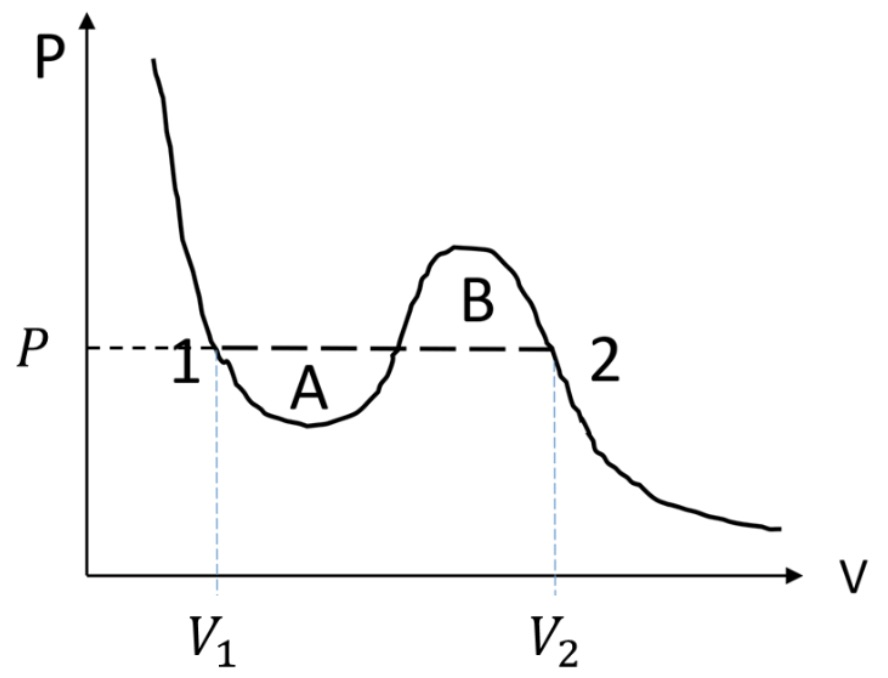
\includegraphics[scale=0.3]{hw2problem4.jpeg}
		\end{center}
		假设上图中虚线1-2表示实际气体-液体共存状态,此状态下温度、压强不变,由
		\[
			dG = -S\,dT + V\,dp
		\]
		可知,Gibbs势不变,则有:
		\[
			G_1 = F_1 + pV_1 = G_2 = F_2 + pV_2.
		\]
		则有:
		\[
			F_2 - F_1 = -\int_{V_1}^{V_2}p\,dV = p(V_1 - V_2).
		\]
		即区域A的面积等于区域B的面积,即证明了Maxwell法则。
	\end{proof}
\end{enumerate}



\end{document}